
\documentclass[a0,portrait]{a0poster}

\usepackage{colordvi,amsmath,epsfig,float,color,multicol} % times

\pagestyle{empty}
\setlength{\parindent}{0cm}
\setlength{\parskip}{2ex}
\setlength{\columnsep}{3cm}
\addtolength{\textwidth}{2cm}
\addtolength{\oddsidemargin}{-1.5cm}

\renewcommand{\normalsize}{\Large}
\def\regularsize{\@setfontsize\normalsize{34pt}{37}}

\renewcommand\refname{}
\setlength{\fboxrule}{0.1cm}


% ----------------------------------------------------------------


% PMS287 CMYK=[100% 69% 0% 11.5%] RGB=[38/256 67/256 151/256]
\definecolor{qmuldarkblue}{rgb}{0.1484375,0.26171875,0.58984375}
\definecolor{emphasisered}{rgb}{0.4921,0.132812,0.164062}

\definecolor{backgrey}{rgb}{0.93,0.93,0.93}
\definecolor{backblue}{rgb}{0.93,0.93,1}
\definecolor{backyellow}{rgb}{1,1,0.88} 

\definecolor{backred}{rgb}{1,0.9,0.9} 
\definecolor{backgreen}{rgb}{0.9,1,0.9}
\definecolor{backpink}{rgb}{1,0.9,1} 
\definecolor{backturquoise}{rgb}{0.9,1,1} 




% ----------------------------------------------------------------


\makeatletter
\renewcommand{\section}{\@startsection
        {section}                          % the name 
        {1}                                % the level
        {0mm}                              % the indent
        {-0.7\baselineskip}                % the beforeskip
        {5mm}                              % the afterskip
        {\center\Huge\color{qmuldarkblue}\bfseries}} % the style
\makeatother

\usepackage{ragged2e} % full justification of reference
\usepackage{enumitem} % compacter itemize
\usepackage{array} % align vertically

\usepackage[framemethod=tikz]{mdframed}
\definecolor{backblue}{rgb}{0.93,0.93,1}
\definecolor{backred}{rgb}{1,0.9,0.9} 
\definecolor{qmulheaderblue}{rgb}{0.1484375,0.26171875,0.58984375}
\definecolor{emphasisered}{rgb}{0.4921,0.132812,0.164062}
\mdfdefinestyle{customSt}{
	innertopmargin=40pt,
	innerbottommargin=30pt,
	innerleftmargin = 15pt,
	innerrightmargin = 15pt,
	leftmargin = 15 pt,
	middlelinecolor = qmulheaderblue,
	middlelinewidth = 3pt,
	backgroundcolor = backblue,
	roundcorner = 20pt
}

\mdfdefinestyle{emphSt}{
	innertopmargin=40pt,
	innerbottommargin=30pt,
	innerleftmargin = 15pt,
	innerrightmargin = 15pt,
	leftmargin = 15 pt,
	middlelinecolor = emphasisered,
	middlelinewidth = 3pt,
	backgroundcolor = backred,
	roundcorner = 20pt
}

\mdfdefinestyle{headerSt}{
	innertopmargin=5pt,
	innerbottommargin=5pt,
	innerleftmargin = 15pt,
	%innerrightmargin = 15pt,
	leftmargin = 15 pt,
	middlelinecolor = qmulheaderblue,
	middlelinewidth = 25pt,
	backgroundcolor = qmulheaderblue,
	roundcorner = 20pt
}

\begin{document}
\begin{mdframed}[style=headerSt]

\begin{center}
\colorbox{qmuldarkblue}
{
 \color{white}

 \parbox{1.0\textwidth}
 {
  \parbox{0.2\textwidth}
  {
   \begin{center}
   
\epsfig{file=img/logos/qmulblue.eps,width=12cm}\\[1ex]
   \textrm
   {
    \footnotesize
    School of Electronic Engineering and Computer Science\\
    Queen Mary University of London\\
   }
   \end{center}
  }
  \parbox{0.58\textwidth}
  {
   \vspace{1cm}
   \begin{center}
   \textrm
   {
    {\veryHuge \bf \em Web Audio E valuation Tool:\\ A browser-based listening test framework}\\[1ex]
    {\Large       Nicholas Jillings, David Moffat, Brecht De Man and Joshua D. Reiss}
   }    
   \end{center}
   \vspace{1cm}
  }
  \parbox{0.2\textwidth}
  {
   \begin{center}
   
\epsfig{file=img/logos/c4dmlogoinverted.eps,width=12cm}\\[1ex]
   \textrm
   {
    \small
    n.g.r.jillings@se14.qmul.ac.uk, \{d.j.moffat,b.deman,joshua.reiss\}@qmul.ac.uk\\
    c4dm.eecs.qmul.ac.uk\\
   }
   \end{center}
  }
 }
}
\end{center}

\end{mdframed}


% ----------------------------------------------------------------

% rounded corners?
\centering
\veryHuge
\textbf{\underline{code.soundsoftware.ac.uk/projects/webaudioevaluationtool}}
\normalsize

\begin{multicols}{2}

\begin{mdframed}[style=customSt]
% !TEX root = ../AESposter.tex
\vspace{-0.8cm}
\section{Introduction}

\begin{itemize}%[noitemsep,nolistsep]
	\item Browser-based framework for listening tests using Web Audio API
	\item No proprietary software required, platform independent
	\item Conduct tests locally or remotely
	\item Client-side file treatment for loudness and synchronising
	\item Open source, contributions welcome
	\item Quick, easy, intuitive, powerful
\end{itemize}
\end{mdframed}

\vspace{0.3cm}

\begin{mdframed}[style=customSt]
\vspace{-0.8cm}
\section{Interfaces}

%\vspace{-1.6cm}
\begin{itemize}
\item A range of test interfaces are available
\item Current work is extending number of interfaces
\item {\bf Do you need a specific test interface? Tell us}
\end{itemize}



%\vspace{2cm}

 \resizebox*{\columnwidth}{!}{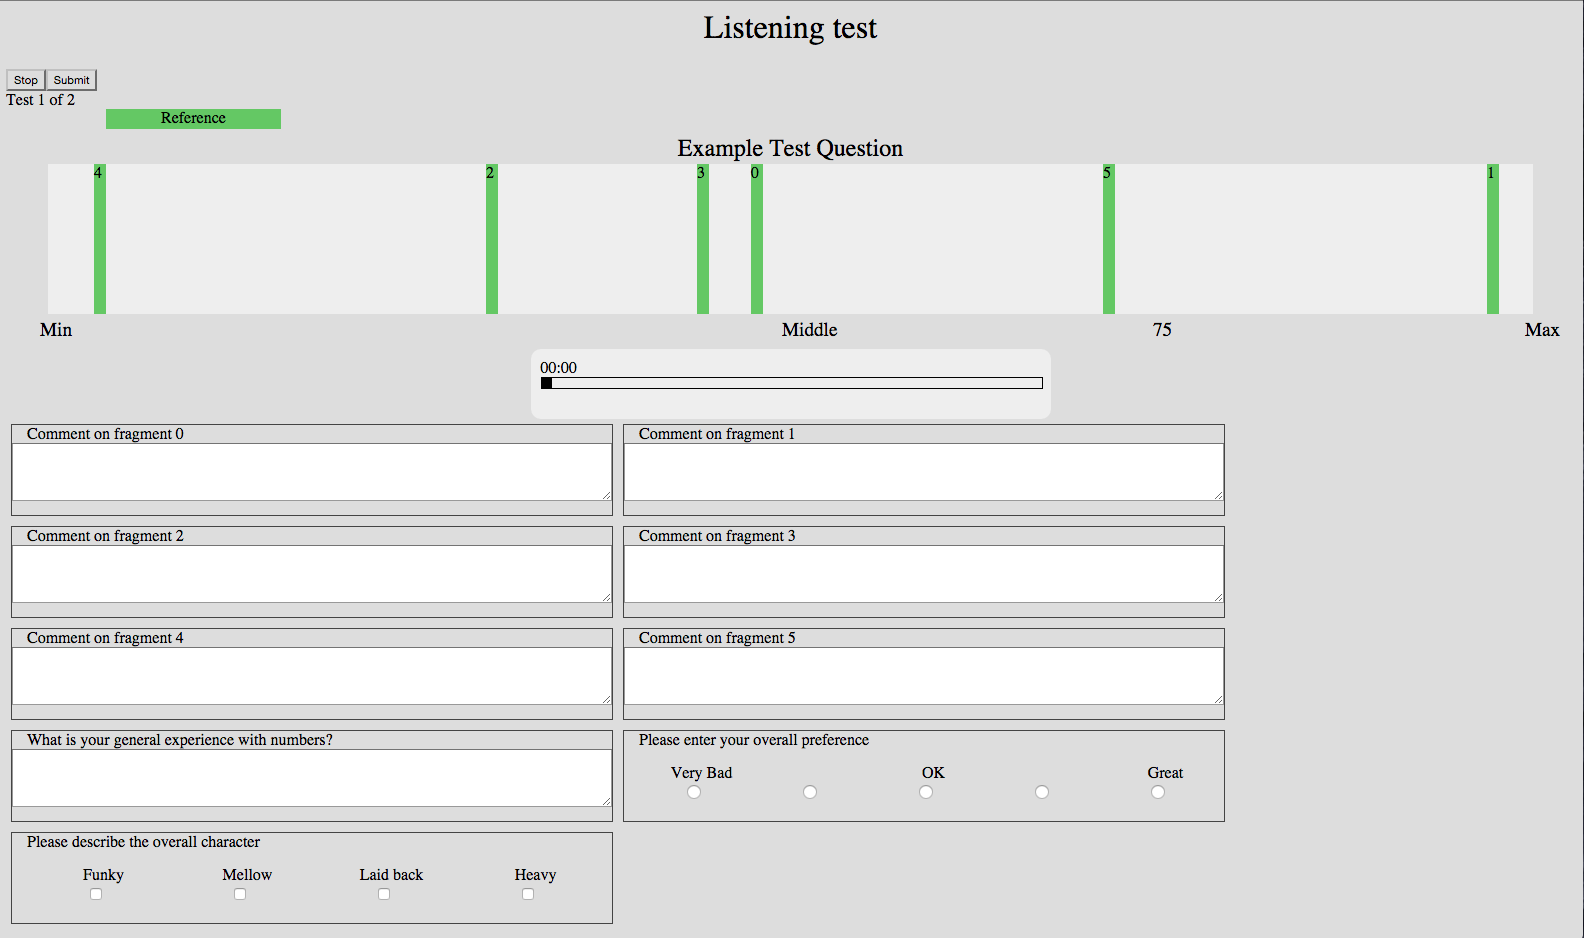
\includegraphics{img/APE}}
 \centering
 \small
 \textbf{APE style test}
 
  \resizebox*{\columnwidth}{!}{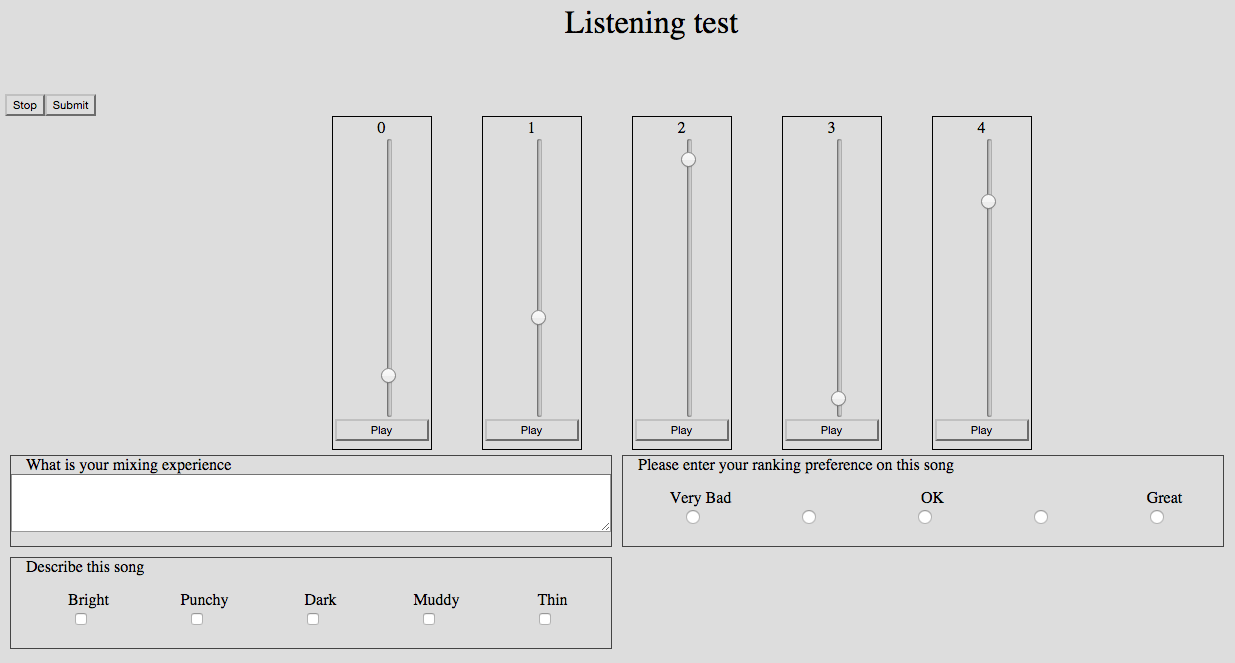
\includegraphics{img/MUSHRA}}
 \centering
 \small
 \textbf{MUSHRA style test}


%\vspace{-1cm}


%\resizebox*{\columnwidth}{!}{\includegraphics{images/blockdiagram.pdf}} 

 \vspace{0.8cm}
\end{mdframed}

%\vspace{.8cm}
%\begin{mdframed}[style=customSt]
%\begin{center}
%\resizebox*{0.35\columnwidth}{!}{
\includegraphics{img/qrcode}}\\
%\end{center}
%\end{mdframed}

\vspace{.8cm}
\begin{mdframed}[style=customSt]
\vspace{-0.8cm}
\section{Infrastructure}

\begin{itemize}[noitemsep,nolistsep]
\item Some information
\item Some information
\item Some information
\item Some information
\end{itemize}
\begin{center}
%\vspace{-2cm}
\resizebox*{\columnwidth}{!}{
\includegraphics{img/logos/soundsoftware_ac_uk_subtitle.eps}}\\
\small
\textbf{Caption for some figure}
\end{center}
\vspace{-1.6cm} \vspace{0.8cm}
\end{mdframed}

\vspace{1cm}

%% THIS GOES BEFORE AN EMPHASISED CELL
%\makeatletter
%\renewcommand{\section}{\@startsection
%        {section}                          % the name 
%        {1}                                % the level
%        {0mm}                              % the indent
%        {-0.7\baselineskip}                % the beforeskip
%        {5mm}                              % the afterskip
%        {\center\Huge\color{emphasisered}\bfseries}} % the style
%\makeatother
%
%\begin{mdframed}[style=emphSt]
%\vspace{-0.8cm}

{\color{emphasisered} \section{Important cell}}

\vspace{-0.8cm}
\huge
\centering
\textbf{b.deman@qmul.ac.uk}

\normalsize

\begin{itemize}%[noitemsep,nolistsep]
	\item Some content
	\item To go in an
	\item Emphasised cell
	\item For some reason
\end{itemize}
\vspace{-1.6cm}

%\resizebox*{0.98\columnwidth}{!}{\includegraphics{images/analysis.pdf}}
%\vspace{-1cm} \vspace{0.8cm}
%\end{mdframed}

% GO BACK TO NORMAL
\makeatletter
\renewcommand{\section}{\@startsection
        {section}                          % the name 
        {1}                                % the level
        {0mm}                              % the indent
        {-0.7\baselineskip}                % the beforeskip
        {5mm}                              % the afterskip
        {\center\Huge\color{qmuldarkblue}\bfseries}} % the style
\makeatother

\vspace{1cm}
\begin{mdframed}[style=customSt]
\vspace{-0.8cm}
\section{Test creation} % or test setup?

\begin{itemize}
	\item Test creation tool to easily build your test
	\begin{itemize}
		\item No need for Programming
	\end{itemize}
	\item or build test in XML
\end{itemize}

\begin{center}
%\vspace{-2cm}
\resizebox*{.8\columnwidth}{!}{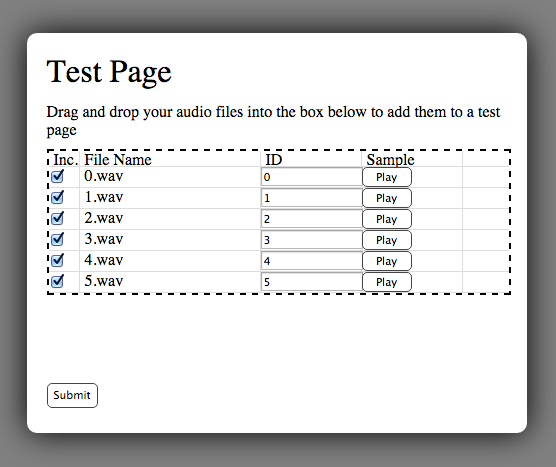
\includegraphics{../WAC2016/img/test_create.png}}\\ % replace with something more meaningful
\small
\textbf{Drag-and-drop audio samples}
\end{center} \vspace{0.8cm}
\end{mdframed}

\vspace{1cm}
\begin{mdframed}[style=customSt]
\vspace{-0.8cm}

{\color{emphasisered} \section{Analysis}}

%\vspace{-0.8cm}
%\huge
%\centering
%\textbf{b.deman@qmul.ac.uk}

\normalsize

\begin{itemize}%[noitemsep,nolistsep]
	\item Includes analysis scripts to quickly present results
	\item Automatic Report Generation
	\item Box Plots, Confidence Plots and Participant Time Line
\end{itemize}
\vspace{-1cm}

\begin{center}
\resizebox*{\columnwidth}{!}{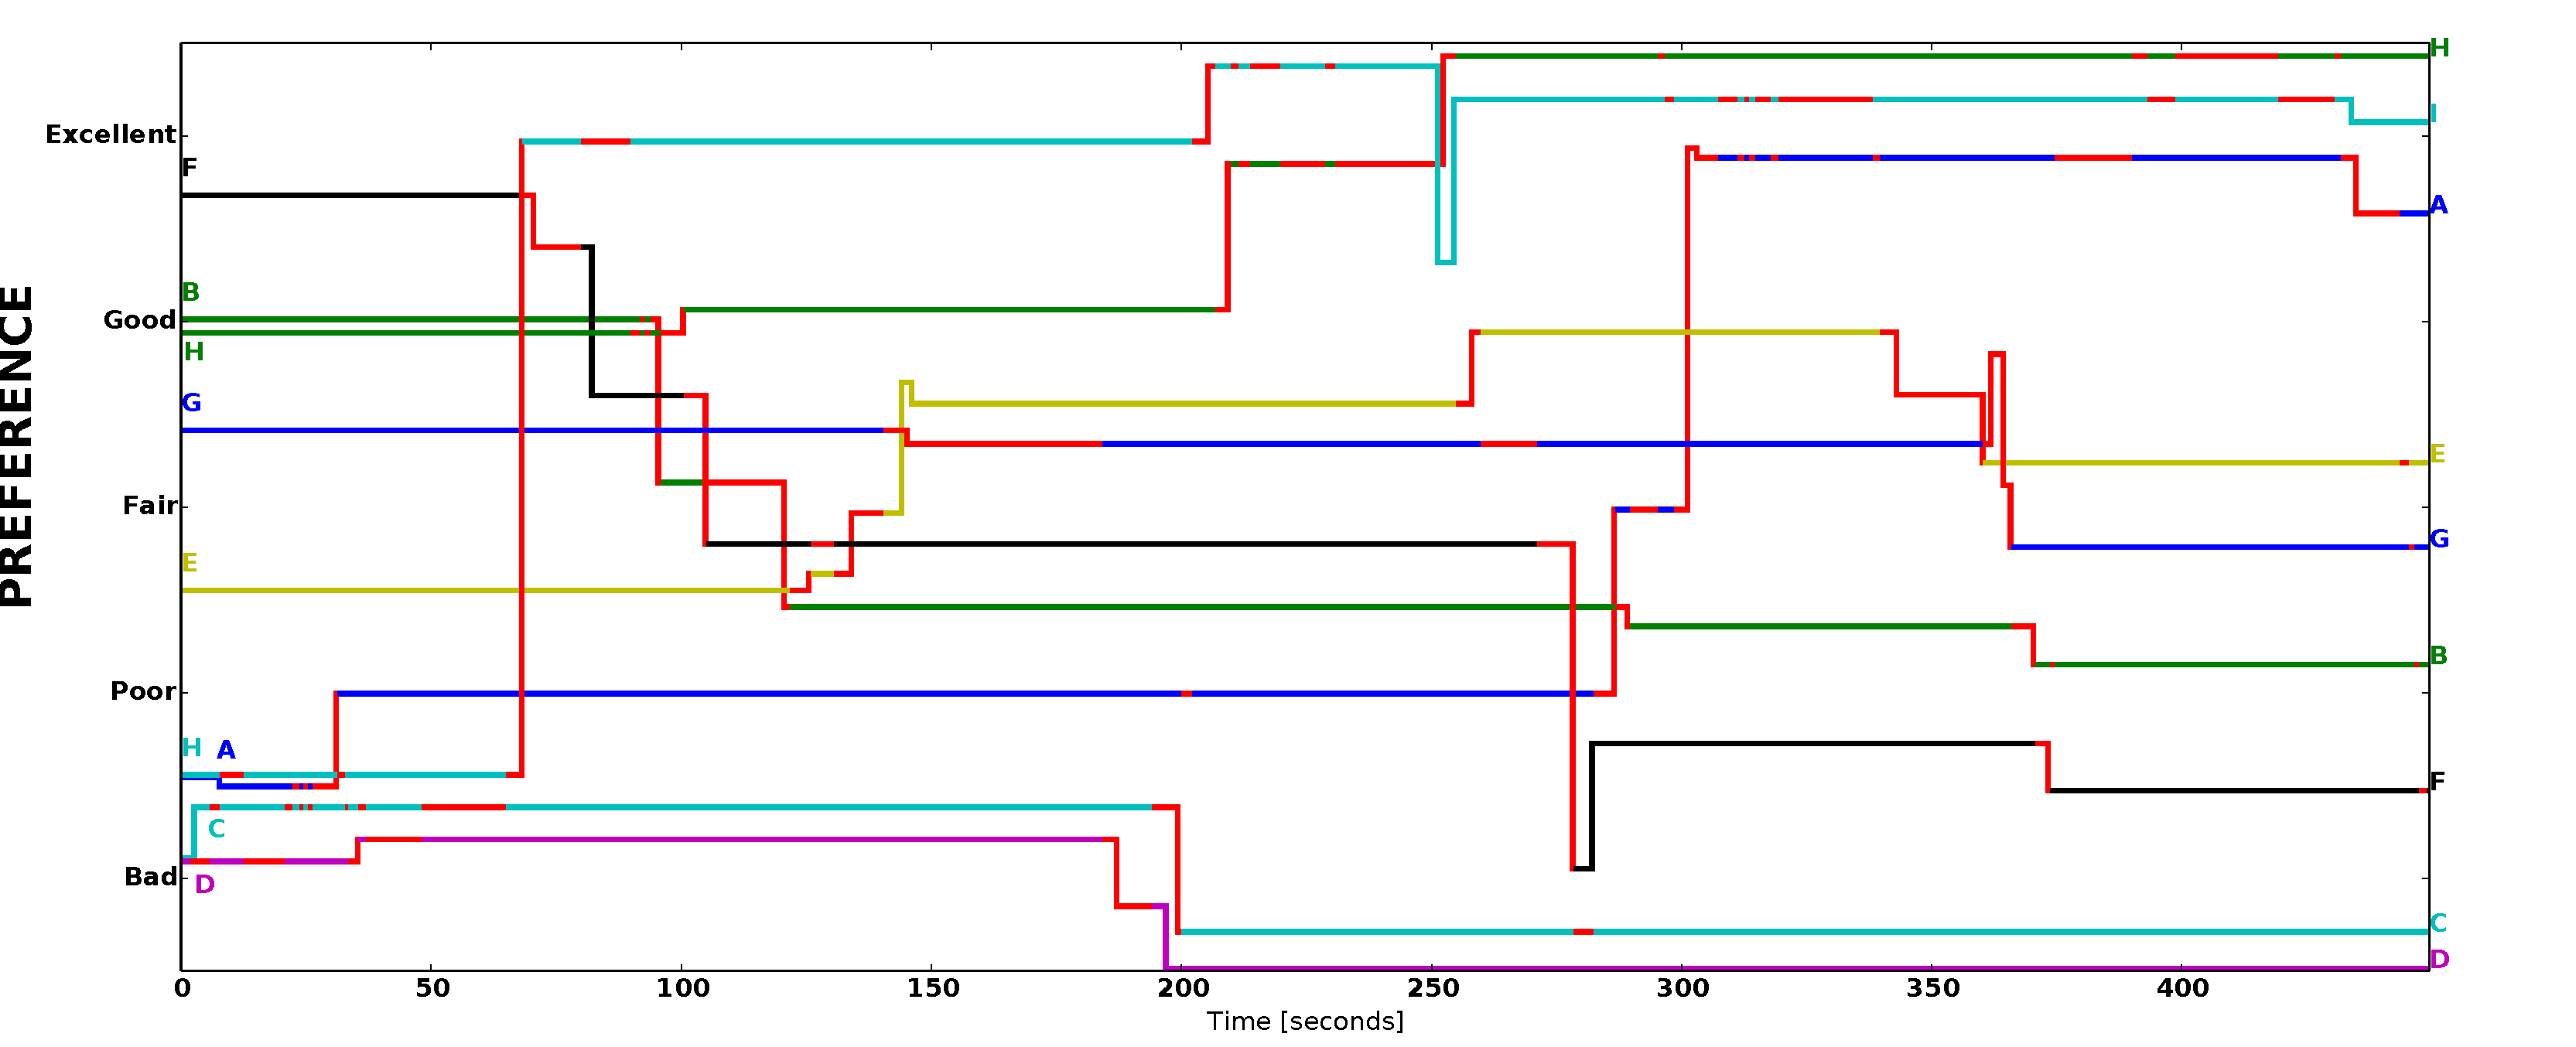
\includegraphics{img/timeline}}
\small
\textbf{Participant Timeline Diagram}
\end{center}

\vspace{-0.3cm}
 \vspace{0.8cm}
\end{mdframed}



\normalsize{\justifying{[1] Nicholas Jillings, Brecht De Man, David Moffat and Joshua D. Reiss, { \it``Web Audio Evaluation Tool: A browser-based listening test environment,''} 12th Sound and Music Computing Conference, July 2015. }\par}

\resizebox*{0.28\columnwidth}{!}{
\includegraphics{img/qrcode}}\\

\end{multicols}


% ----------------------------------------------------------------

\vspace{0.6cm}

\begin{mdframed}[style=headerSt]

\colorbox{qmuldarkblue}
{
 \color{white}
 \parbox{\textwidth}
 {
%  \vspace{0.5cm}

  \begin{center}

  
\textbf{DMRN+10}: Digital Music Research Network One-day Workshop 2015 at Queen Mary University of London
  % or put nothing here so it's reusable...
  
  \end{center}

  \vspace{-1cm}
 }
}

\end{mdframed}

\end{document}
